\documentclass[11pt,a4paper]{article}
\usepackage[utf8]{inputenc}
\usepackage{geometry}
\usepackage[spanish,activeacute]{babel}
\usepackage{amsmath}
\usepackage{amsfonts}
\usepackage{amsthm}
\usepackage{amssymb}
\usepackage{graphicx}
\usepackage{euler}						% Texto matematico estilo Concrete Mathematics
\usepackage{mathtools}					% \mathclap, \DeclarePairedDelimiter
\usepackage[linesnumbered]{algorithm2e}
\usepackage{hyperref}
\usepackage{float}

\usepackage{mathdots}					% Puntitos en diagonal invertidos

%\SetFuncSty{textsc}

\newtheorem*{teo}{\textbf{Teorema}}
\newtheorem*{prop}{\textbf{Proposición}}
\newtheorem*{coro}{\textbf{Corolario}}
\newtheorem*{lema}{\textbf{Lema}}
\newtheorem*{afir}{\textbf{Afirmación}}

\theoremstyle{definition}
\newtheorem*{defi}{\textbf{Definición}}

\renewcommand{\rmdefault}{pplx}	% Fuente estilo Concrete Mathematics

\SetFuncSty{textsc}

\newcommand\unkeq{\stackrel{\mathclap{\normalfont\mbox{?}}}{=}}
\newcommand\hieq{\stackrel{\mathclap{\normalfont\mbox{HI}}}{=}}
\newcommand{\Oh}[1]{$O(#1)$}

\DeclarePairedDelimiter\ceil{\lceil}{\rceil}
\DeclarePairedDelimiter\floor{\lfloor}{\rfloor}

\author{Guido Tagliavini Ponce}
\title{\LARGE{\textbf{Balanceo de \'arboles y \'arboles AVL}}}
%\date{01/10/2014}

\begin{document}
\hfill 
\includegraphics[scale = 0.75]{imagenes/logo_dc.jpg}~\\[0.25cm]

\begin{center}
	\textbf{\Large Balanceo de \'arboles y \'arboles AVL}\\[1cm]
	{\large Guido Tagliavini Ponce\\[0.15cm]}
	Universidad de Buenos Aires\\[0.15cm]
	\texttt{guido.tag@gmail.com}\\[1cm]
\end{center}
\rule{\linewidth}{0.2mm}
\tableofcontents

%\section{Disclaimer}

%Este apunte se provee como una ayuda adicional; un repaso en castellano de la bibliografía sobre ABBs y AVLs y de las respectivas teóricas. Su lectura no es un reemplazo de ninguna de las anteriores. Si bien es una versi'on estable, est'a en proceso de depuración (agradeceremos reportar al autor cualquier error o sugerencia). Ante cualquier duda, rogamos remitirse a la bibliografía oficial de la materia.

\section{Introducci'on}

La estructura de 'arbol es una idea fundamental en la computaci'on. Su importancia radica en su capacidad para estructurar informaci'on de manera din'amica, es decir, posibilitando  la f'acil realizaci'on de cambios en esa informaci'on a lo largo del tiempo. El concepto de balanceo aparece como una soluci'on al crecimiento desmesurado de la altura de los mismos, lo cual imposibilita realizar operaciones que requieran atravesar el 'arbol desde la ra'iz hasta una hoja, en forma eficiente.

En este trabajo revisamos la noci'on de balanceo, y estudiamos diversas familias de 'arboles que son balanceados. Una de estas familias derivar'a en el concepto de 'arbol AVL. Estos 'arboles son balanceados y permiten ejecutar eficientemente las operaciones de diccionario, lo cual los hace una representaci'on perfecta para estos tipos abstractos de datos. Por esta raz'on, en la segunda parte del trabajo nos concentramos en la implementaci'on detallada de las operaciones de un AVL.

\section{Balanceo de 'arboles}

\subsection{Motivaci'on}

Intuitivamente, que un 'arbol est'e balanceado significa que no hay sub'arboles que sean mucho m'as grandes (en alg'un sentido de \textit{grande}) que otros sub'arboles. Una interpretaci'on gr'afica de esto es que un 'arbol balanceado es \textit{llano}. Los 'arboles que cumplen esta noci'on intuitiva de balanceo por excelencia, son los completos (aquellos que tienen todos los niveles completos), puesto que su altura es chica en relaci'on a la cantidad de nodos que concentra entre todos sus niveles. El hecho de que un 'arbol binario completo de $n$ nodos tiene altura aproximadamente $\lg n$, motiva la definici'on central de todo este apunte.

\begin{defi}
Un 'arbol de $n$ nodos se dice \textit{balanceado} si su altura es \Oh{\lg n}
\end{defi}

Retomando la discusi'on de la introducci'on, la utilidad pr'actica de los 'arboles balanceados aparece cuando se combina este concepto con el de 'arbol de b'usqueda. Recordemos qu'e significa esto 'ultimo.

\begin{defi}
Un 'arbol binario con claves en los nodos se dice \textit{de b'usqueda} (y escribimos ABB) si:
\begin{itemize}
	\item toda clave en el sub'arbol izquierdo es menor que la clave de la ra'iz;
	\item toda clave en el sub'arbol derecho es mayor que la clave de la ra'iz;
	\item tanto el sub'arbol izquierdo como el derecho son 'arboles binarios de b'usqueda. 
\end{itemize}
\end{defi}

Un ABB permite determinar la existencia de una clave en el 'arbol en tiempo proporcional a la altura del 'arbol \cite{cormen01}. En un ABB de $n$ nodos cualquiera, esto puede ser, en el peor caso, \Oh{n}. Sin embargo, si el 'arbol es balanceado, su altura ser'a $O(\lg n)$, con lo cual el costo de la b'usqueda baja a $O(\lg n)$.

Nuestro objetivo ser'a definir familias de 'arboles binarios que sean balanceados. Como hemos mostrado, nuestro inter'es se centra en 'arboles que puedan ser usados como estructuras de representaci'on de diccionarios, por lo que una propiedad deseada para estas familias es que al ser utilizados como ABBs, soporten la inserci'on y el borrado de nodos (es decir, la actualizaci'on a lo largo del tiempo), de modo tal que al efectuar tales operaciones se obtenga otro 'arbol de la familia de 'arboles balanceados. %Esta 'ultima propiedad es lo que nos permitir'a asegurar que a lo largo de una secuencia de operaciones, los costos de inserci'on, borrado y b'usqueda se mantienen. Esto quedar'a m'as claro y resultar'a evidente al ver ejemplos concretos.

\subsection{'Arboles binarios completos}

Como hemos visto, los 'arboles binarios completos son una familia de 'arboles balanceados elemental. El hecho de que sean balanceados se fundamenta en el siguiente resultado, al que ya hemos hecho alusi'on.

\begin{teo}
Un 'arbol binario completo $T$ de $n$ nodos tiene altura $\lg(n + 1)$.

\begin{proof}
Sea $h$ la altura de $T$. Como $T$ es completo, los $h$ niveles de $T$ est'an completos, es decir que

\[n = \sum_{i = 0}^{h - 1}2^i = 2^h - 1\]
\end{proof}
\end{teo}

\begin{coro}
Un 'arbol binario completo es balanceado.
\end{coro}

El problema con esta clase de 'arboles, es que son extremadamente r'igidos, en el sentido que no es posible realizar una inserci'on o borrado de un nodo y obtener otro 'arbol completo, como muestra la figura \ref{fig3}.

\begin{figure}[h]
	\begin{center}
	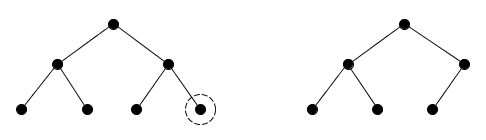
\includegraphics[scale=0.6]{imagenes/fig3.jpg}
	\end{center}
	\caption{un 'arbol binario completo deja de ser completo al eliminarle un nodo}
	\label{fig3}
\end{figure}

\subsection{Balanceo perfecto}

Necesitamos relajar un poco esta rigidez de los 'arboles completos. Observemos que una caracter'istica de un 'arbol completo es que todas sus hojas estan en el 'ultimo o en el ante'ultimo nivel. Obviamente, esta propiedad caracteriza a muchos otros 'arboles que no son completos, como muestra la figura \ref{fig1}. Para evitar casos de extremo desbalanceo, como el de la figura, pediremos que no haya nodos que tengan un s'olo hijo, que se puede ver que son los que abundan en el ejemplo, y que causan que existan ramas largas.

\begin{figure}[h]
	\begin{center}
	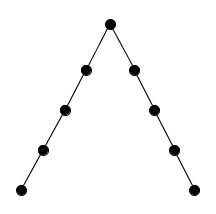
\includegraphics[scale=0.6]{imagenes/fig1.jpg}
	\end{center}
	
	\caption{'arbol que tiene sus hojas al mismo nivel, pero no es balanceado}
	\label{fig1}
\end{figure}

Con todo esto en mente, vamos a definir un nuevo criterio de balanceo, que no es m'as que una serie de restricciones sobre 'arboles binarios que definen una familia.

\begin{defi}
	Un 'arbol binario se dice \textit{lleno} si todo nodo tiene 0 o 2 hijos.
\end{defi}

\begin{defi}
	Un 'arbol binario se dice \textit{perfectamente balanceado} si:
	\begin{itemize}
		\item es un 'arbol lleno;
		\item todas sus hojas se encuentran en el 'ultimo 'o ante'ultimo nivel.
	\end{itemize}
\end{defi}

La figura \ref{fig2} muestra un 'arbol binario perfectamente balanceado. Notar que tiene forma achatada, condici'endose, intuitivamente, con la noci'on de balanceo. El siguiente resultado expresa formalmente esto 'ultimo.

\begin{figure}[h]
	\begin{center}
	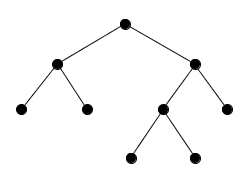
\includegraphics[scale=0.6]{imagenes/fig2.jpg}
	\end{center}
	\caption{'arbol perfectamente balanceado}
	\label{fig2}
\end{figure}

\begin{teo}
	Un 'arbol binario perfectamente balanceado $T$ de $n$ nodos tiene altura $\ceil{\lg(n + 1)}$.
\begin{proof}
	Sea $h$ la alura de $T$. Lo primero que veremos es que cada nivel $0 \leq i < h - 1$ est'a completo. En efecto, si suponemos que $i > 0$ es el primer nivel que no est'a completo, entonces existe un nodo $v$ en el nivel $i - 1$ que no tiene dos hijos, dado que el $i - 1$ est'a completo. Como $T$ es un 'arbol lleno, entonces $v$ debe tener 0 hijos, es decir que es una hoja. Luego, $T$ tiene una hoja en el nivel $i - 1 < h - 2$, lo cual contradice al hecho de que todas las hojas de dicho 'arbol est'an en el nivel $h - 1$ 'o $h - 2$.
	
	Por lo anterior, debe ser
	
	\[n > \sum_{i = 0}^{h - 2} 2^i = 2^{h - 1} - 1\]
	
	La desigualdad es estricta debido a que $T$ tiene al menos un nodo en el nivel $h - 1$.
	Por otro lado, como $T$ tiene altura $h$, se tiene
	
	\[n \leq \sum_{i = 0}^{h - 1} 2^i = 2^h - 1\]
	
	Juntando ambas desigualdades,
	
	\[2^{h - 1} - 1 < n \leq 2^h - 1\]
	
	Sumando 1 y tomando logaritmos,
	
	\[h - 1 < \lg(n + 1) \leq h\]
	
	Es decir que $h = \ceil{\lg(n + 1)}$.
	
\end{proof}
\end{teo}

\begin{coro}
	Un 'arbol binario perfectamente balanceado es balanceado.
\end{coro}

Lamentablemente, esta familia de 'arboles balanceados sigue padeciendo algunos de los problemas que tienen los 'arboles binarios completos. Particularmente sufre el problema de que no hay 'arboles perfectamente balanceados para cada cantidad de nodos posible. La figura \ref{fig4} muestra un ejemplo.

\begin{figure}[h]
	\begin{center}
	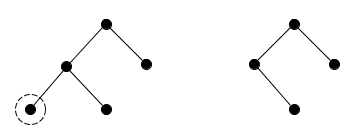
\includegraphics[scale=0.6]{imagenes/fig4.jpg}
	\end{center}
	\caption{'arbol binario perfectamente balanceado deja de ser perfectamente balanceado al eliminar un nodo}
	\label{fig4}
\end{figure}

\subsection{Balanceo en altura}

\begin{defi}
	Un 'arbol binario se dice \textit{balanceado en altura} si para cada nodo, la altura de su sub'arbol derecho e izquierdo difieren a lo sumo en una unidad.
\end{defi}

\begin{teo}
	Un 'arbol binario balanceado en altura es balanceado.
	
\begin{proof}
	La pregunta clave de la demostraci'on es,
	
	\begin{center}
	\textit{¿cu'al es la m'inima cantidad de nodos que puede tener un 'arbol binario balanceado en altura, de altura $h$?}
	\end{center}
	
	Intuitivamente, responder a esta pregunta es 'util porque fijado un 'arbol balanceado en altura de $n$ nodos y altura $h$, dicho 'arbol no puede ser demasiado ralo. Matem'aticamente, $n$ debe ser suficientemente grande,z respecto de $h$. M'as precisamente, $n$ debe estar acotado inferiormente por una funci'on de $h$. Esto se debe a que el balance deber'ia obligar a que haya una gran cantidad de nodos concentrados a lo largo de los $h$ niveles.

	%Sabiendo esto podremos acotar inferiormente a la cantidad de nodos de un 'arbol, por la cantidad m'inima de nodos que puede tener un 'arbol de su altura.
	
	Llamemos $n_{min}(h)$ a la m'inima cantidad de nodos de un 'arbol binario balanceado de altura $h$. Es claro que $n_{min}(1) = 1$ y $n_{min}(2) = 2$. Si $h > 2$, ¿cu'anto vale $n_{min}(h)$? Un 'arbol binario balanceado en altura de $n$ nodos y altura $h > 2$ debe tener dos sub'arboles, izquierdo y derecho. De la definici'on de balanceo en altura se deduce que estos dos tambi'en son balanceados en altura. Como $T$ tiene altura $h$, entonces uno de ellos tiene altura $h - 1$, y el otro altura $h - 1$ o $h - 2$, puesto que la diferencia entre las alturas de los mismos es a lo sumo 1. Gr'aficamente, la situaci'on es la siguiente:
	
\begin{figure}[H]
	\begin{center}
	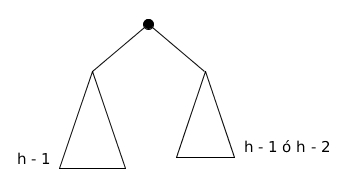
\includegraphics[scale=0.6]{imagenes/figdembh.jpg}
	\end{center}
\end{figure}

	
	Luego,
	
	\[n \geq 1 + n_{min}(h - 1) + \min(n_{min}(h - 1), n_{min}(h - 2))\]
	
Como $T$ es arbitrario de altura $h$, resulta que $n_{min}(h) \geq 1 + n_{min}(h - 1) + \min(n_{min}(h - 1), n_{min}(h - 2))$. De esta desigualdad, m'as los casos base, se sigue inmediatamente que $n_{min}(h) > n_{min}(h - 1)$ para todo $h > 1$, con lo cual la expresi'on anterior se simplifica a

\[n_{min}(h) \geq 1 + n_{min}(h - 1) + n_{min}(h - 2)\]

Para probar la igualdad, basta ver que hay alg'un 'arbol binario balanceado en altura, de altura $h$, con cantidad de nodos $1 + n_{min}(h - 1) + n_{min}(h - 2)$. Este 'arbol se puede construir f'acilmente en forma inductiva, razonando igual que antes. En definitiva,

\[n_{min}(h) = 1 + n_{min}(h - 1) + n_{min}(h - 2)\]

Observemos que esta recurrencia tiene un parecido con la sucesi'on de Fibonacci. La siguiente tabla muestra los primeros valores de $n_{min}$ y $Fib$.

\begin{center}
\begin{tabular}{|c|c|c|}
\hline
$h$ & $n_{min}(h)$ & $Fib(h)$\\
\hline
\hline
1 & 1 & 1\\
2 & 2 & 1\\
3 & 4 & 2\\
4 & 7 & 3\\
5 & 12 & 5\\
6 & 20 & 8\\
7 & 33 & 13\\
8 & 54 & 21\\
\hline
\end{tabular}
\end{center}

Queda como ejercicio para el lector probar que $n_{min}(h) = Fib(h + 2) - 1$. Dado que $Fib(k) = \Omega(\phi^k)$, tenemos $n_{min}(h) = \Omega(\phi^h)$, donde $\phi = \frac{1 + \sqrt{5}}{2}$ es el n'umero 'aureo.

Finalmente, tomemos un 'arbol binario balanceado en altura de $n$ nodos y altura $h$, y veamos que $h = O(\lg n)$. Se tiene $n \geq n_{min}(h) = \Omega(\phi^h)$, con lo cual $n = \Omega(\phi^h)$. Pero entonces $h = O(\log_{\phi} n) = O(\lg n)$.
\end{proof}
\end{teo}

Como veremos en la segunda parte de este trabajo, esta familia de 'arboles binarios balanceados ha probado ser 'util.

\subsection{Balanceo en peso}

El 'ultimo criterio de balanceo que estudiaremos no es una propuesta superadora del balanceo en altura. A'un as'i, es interesante conocerlo, sencillamente con el fin de reforzar la idea de que hay diversas propiedades que se le pueden exigir a un 'arbol de manera tal de asegurar su balance, aunque no todas son igualmente 'utiles debido a su mayor o menor flexibilidad.

\begin{defi}
	Un 'arbol se dice \textit{balanceado en peso} si para cada nodo, la cantidad de nodos en su sub'arbol derecho e izquierdo difieren a lo sumo en una unidad.
\end{defi}

\begin{teo}
	Un 'arbol binario balanceado en peso $T$ de $n$ nodos tiene altura $\ceil{\lg(n + 1)}$.

\begin{proof}
	Sea $h$ la altura de $T$. Veamos, primero, que al igual que los 'arboles binarios perfectamente balanceados, esta clase de 'arboles tienen cada nivel $0 \leq i < h - 1$ completo. Procedemos por inducci'on en $h$.
	El caso $h = 1$ es trivial. Sea $h > 1$. Sea $r$ la ra'iz de $T$. Si $r$ tiene un 'unico hijo entonces $T$ s'olo puede estar compuesto por $r$ y su hijo, puesto que es balanceado en peso, con lo cual vale el resultado. Supongamos que $r$ tiene dos hijos. Entonces, $r$ tiene un sub'arbol izquierdo $L$ y uno derecho $R$, con alturas $h_L$ y $h_R$ respectivamente, y tama\~nos $n_L$ y $n_R$ respectivamente. Gr'aficamente este 'arbol tiene la siguiente forma:
	
\begin{figure}[H]
	\begin{center}
	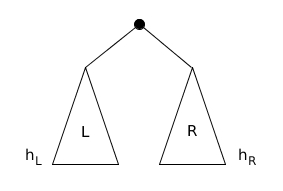
\includegraphics[scale=0.6]{imagenes/figdembp.jpg}
	\end{center}
\end{figure}

	Como $T$ es balanceado, se tiene
	
\begin{equation}
	|n_R - n_L| \leq 1	
\end{equation}

	M'as a'un, tanto $L$ como $R$ son balanceados en peso. Como adem'as ambos tienen altura menor que $h$, vale la hip'otesis inductiva sobre ellos, con lo cual $L$ y $R$ tienen todo nivel completo, excepto, quiz'as, el 'ultimo.
	
	Como $T$ tiene altura $h$ entonces podemos suponer, sin p'erdida de generalidad, que $h_L = h - 1$. Como $L$ tiene los primeros $h - 2$ niveles completos, vale
	
\[n_L > \sum_{i = 0}^{h - 3} 2^i = 2^{h - 2} - 1\]

	La desigualdad es estricta porque $L$ tiene al menos un nodo en el nivel $h - 2$. En definitiva

\begin{equation}
	n_L \geq 2^{h - 2}
\end{equation}	

	 De la ecuaci'on (1) se deduce que $n_R \geq n_L - 1$. Juntando esto con (2) resulta que 

\begin{equation}
	n_R \geq 2^{h - 2} - 1
\end{equation}	
	
	Como $R$ tiene altura $h_R$, entonces $n_R \leq 2^{h_R - 1} - 1$. Combinando esto 'ultimo con (3),
	
\[2^{h - 2} - 1 \leq 2^{h_R - 1} - 1\]

Luego $h_R \geq h - 1$, pero como $h_R$ tiene altura a lo sumo $h - 1$, debe ser $h_R = h - 1$. En definitiva, ambos sub'arboles de $r$ tienen la misma altura $h - 1$ y tienen todos sus niveles completos, salvo quiz'as el 'ultimo, lo cual prueba lo que quer'iamos y concluye la inducci'on.

A partir de aqu'i se procede igual que en el caso del balanceo perfecto.

\end{proof}
\end{teo}

\section{'Arboles AVL}

\begin{defi}
	Un 'arbol AVL es un ABB balanceado en altura.
\end{defi}

El nombre de estos 'arboles proviene de las iniciales de sus dos creadores, Adelson-Velskii y Landis, y fue el primer ABB balanceado publicado en la historia. En esta segunda parte del trabajo, veremos c'omo estos 'arboles permiten implementar las operaciones de diccionario, todas en tiempo logar'itmico, gracias a la noci'on de balanceo que utilizan.

Un concepto central a la hora de hablar de balanceo en altura es el siguiente.

\begin{defi}
	Se define el factor de balanceo de un nodo $v$ de un 'arbol binario como
	
	\[fb(v) = \text{altura del sub'arbol derecho de }v - \text{altura del sub'arbol izquierdo de }v\]
\end{defi}

Por lo tanto, un 'arbol binario es balanceado en altura si para cada nodo $v$, vale $|fb(v)| \leq 1$. Entonces, cada nodo de un AVL tendr'a un factor de balanceo 0, 1 'o $-1$.

Como ya hemos dicho, las dos operaciones que buscamos soportar son las de b'usqueda, inserci'on y borrado de claves. Dado que un AVL es, en particular, un ABB, la b'usqueda sobre estos 'arboles es exactamente igual a la b'usqueda sobre ABBs, y tendremos asegurado un costo logar'itmico gracias al balanceo. Para la inserci'on y borrado, el esquema de las operaciones ser'a el siguiente:

\begin{enumerate}
	\item Realizar la operaci'on como en un ABB cl'asico.
	\item Rebalancear aquellos nodos desbalanceados.
\end{enumerate}

En este documento no profundizamos sobre las operaciones cl'asicas sobre ABBs, de modo que el lector interesado puede remitirse a \cite{cormen01}. De cualquier manera, a efectos de entender el funcionamiento de un AVL no podemos abstraernos completamente del funcionamiento de tales operaciones cl'asicas de ABB. Necesitaremos hacer uso de algunos hechos que enunciaremos en su debido momento.

Las figuras \ref{fig5} y \ref{fig6} muestran por qu'e es necesario realizar el paso 2, luego de una inserci'on o un borrado. En la figura \ref{fig5}, el ABB inicialmente posee todos sus nodos balanceados, pero despu'es de insertar la clave -15, el nodo de clave -1 pasa a tener factor de balanceo -2. En la figura \ref{fig6}, partimos del mismo 'arbol AVL y al borrar la clave 5, el nodo de clave 2 pasa a tener factor de balanceo -2.

\begin{figure}[h]
	\begin{center}
		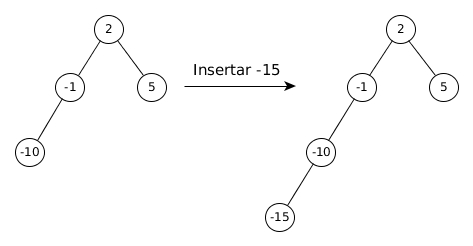
\includegraphics[scale=0.6]{imagenes/fig5.jpg}
	\end{center}
	\caption{desbalanceo de un nodo en una inserci'on}
	\label{fig5}
\end{figure}

\begin{figure}[h]
	\begin{center}
		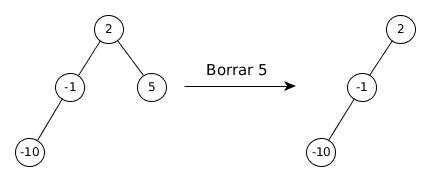
\includegraphics[scale=0.6]{imagenes/fig6.jpg}
	\end{center}
	\caption{desbalanceo de un nodo en un borrado}
	\label{fig6}
\end{figure}


\subsection{Rotaciones en ABBs}

Para remendar los nodos desbalanceados, realizaremos sobre ciertos nodos una serie de operaciones que se conocen como \textit{rotaciones}. Dado que nuestro objetivo es recuperar la condici'on de AVL, necesitamos no s'olo arreglar los factores de balanceo, sino tambi'en mantener el invariante de ABB.

Para restaurar el balanceo, utilizaremos 'unicamente dos tipos de operaciones de rotaci'on, que se ilustran en la figura \ref{fig7}. Notar que estas operaciones son independientes de cualquier noci'on de balanceo, y que son aplicables en cualquier ABB, puesto que preservan el invariante de representaci'on de estos 'arboles. En otras palabras, al aplicar cualquiera de las rotaciones a un ABB, el resultado es otro ABB.

\begin{figure}[H]
	\begin{center}
		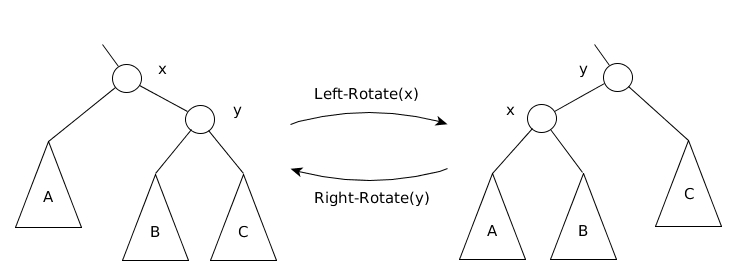
\includegraphics[scale=0.6]{imagenes/fig7.jpg}
	\end{center}
	\caption{rotaciones en ABBs}
	\label{fig7}
\end{figure}

Las dos operaciones son una inversa de la otra. Por un lado, \textsc{Left-Rotate}($x$) toma un nodo $x$, que debe tener un hijo derecho $y$, rotando hacia la izquierda a $x$, dejando a $y$ como ra'iz del sub'arbol, y colgando a la derecha de $x$ el sub'arbol izquierdo de $y$ (si hubiera uno). Observar que al rotar a $x$ a la izquierda, estamos \textit{bajando} a este nodo y \textit{levantando} al nodo $y$.

Por otro lado, \textsc{Right-Rotate}($y$) exige que $y$ tenga un hijo izquierdo, y realiza una operaci'on an'aloga, en forma espejada. En este caso, es al nodo $y$ que rotamos hacia la derecha, haciendo que \textit{baje} y, consecuentemente, que \textit{suba} su hijo izquierdo $x$.

Intuitivamente, utilizaremos \textsc{Left-Rotate}($x$) para trasladar un poco del \textit{peso} del sub'arbol derecho hacia el izquierdo, y \textsc{Right-Rotate}($y$), contrariamente, para llevar peso del sub'arbol izquierdo hacia el derecho. Aqu'i cuando hablamos de peso, no nos referimos a una cantidad de nodos sino a una altura, que es aquello que intentamos balancear.

\subsection{Casos de desbalanceo}

Al realizar una inserci'on o borrado y encontrarnos con que algunos factores de balanceo son estrictamente mayores que 1, resulta conveniente resolver cada uno de estos problemas progresivamente, rebalanceando los nodos m'as profundos, continuando hacia los m'as cercanos a la ra'iz. Por esta raz'on, es 'util plantearse los distintos escenarios en los que tenemos un sub'arbol cuya ra'iz est'a desbalanceada en una unidad (es decir, tiene factor de balanceo -2 'o 2), pero tal que todo otro nodo debajo de dicho nodo est'a balanceado.

Llamemos $p$ a la ra'iz de un tal sub'arbol. Concentr'emonos, primero, en el caso $fb(p) = 2$. Supongamos que el sub'arbol izquierdo de $p$ tiene altura $h$. Entonces, el sub'arbol derecho de $p$ tiene altura $h + 2$. Este sub'arbol derecho debe tener al menos dos nodos, con lo cual podemos nombrar $q$ a su ra'iz. La figura \ref{fig8} muestra la estructura de este 'arbol. A partir de ahora, los n'umeros dentro de cada nodo representar'an los factores de balanceo de los mismos.

\begin{figure}[H]
	\begin{center}
		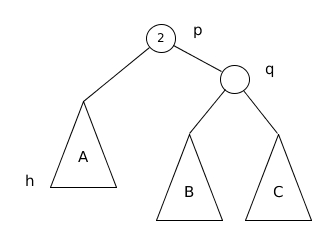
\includegraphics[scale=0.6]{imagenes/fig8.jpg}
	\end{center}
	\caption{$fb(p) = 2$}
	\label{fig8}
\end{figure}

Dividimos nuevamente en casos, seg'un el valor de $fb(q)$. Como asumimos que todos los nodos debajo de $p$ est'an balanceados, debe ser $fb(q) \in \{-1, 0, 1\}$.

Supongamos $fb(q) = 1$. Observar que esto determina las alturas de ambos sub'arboles de $q$. Como el sub'arbol derecho de $p$ es mucho m'as alto que el izquierdo, debemos realizar alg'un tipo de rotaci'on que traslade peso desde la derecha hacia la izquierda. Por este motivo, parece razonable ejecutar una \textsc{Left-Rotate}($p$), y como muestra la figura \ref{fig9}, esta operaci'on reestablece el balance.

\begin{figure}[H]
	\begin{center}
		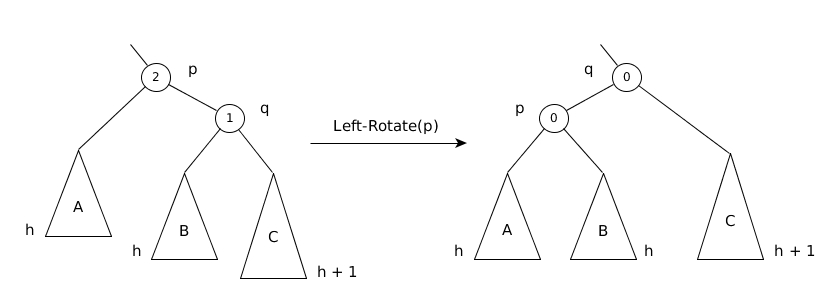
\includegraphics[scale=0.55]{imagenes/fig9.jpg}
	\end{center}
	\caption{$fb(p) = 2$ y $fb(q) = 1$ \textbf{(caso A)}}
	\label{fig9}
\end{figure}

Supongamos $fb(q) = 0$. Utilizando la misma estrategia de rotar $p$ hacia la izquierda, vemos que nuevamente logramos rebalancear el sub'arbol, como muestra la figura \ref{fig10}.

\begin{figure}[H]
	\begin{center}
		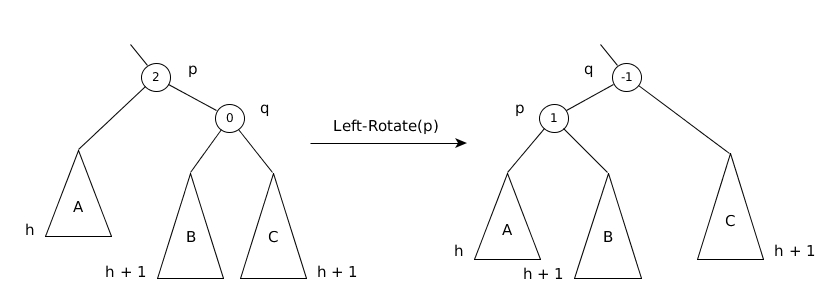
\includegraphics[scale=0.55]{imagenes/fig10.jpg}
	\end{center}
	\caption{$fb(p) = 2$ y $fb(q) = 0$ \textbf{(caso B)}}
	\label{fig10}
\end{figure}

Finalmente, supongamos $fb(q) = -1$. Podemos intentar otra vez la rotaci'on de $p$ hacia la izquierda, aunque lamentablemente esto funciona, pues terminaremos con $fb(q) = -2$, como se ve en la figura \ref{fig11}. Necesitamos rebalancear con m'as cuidado.

\begin{figure}[H]
	\begin{center}
		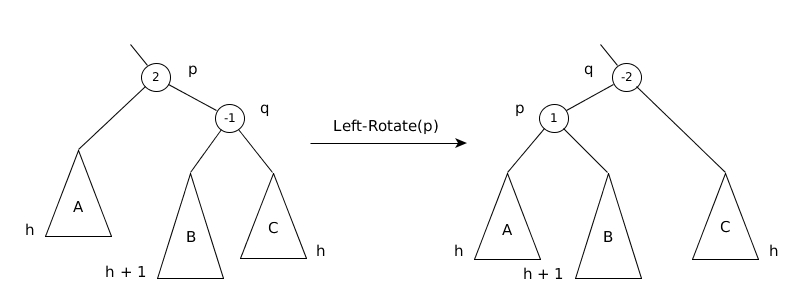
\includegraphics[scale=0.55]{imagenes/fig11.jpg}
	\end{center}
	\caption{rotar $p$ hacia la izquierda falla}
	\label{fig11}
\end{figure}

Notemos que el sub'arbol $B$, que es el m'as pesado de los sub'arboles de $q$, es el que impide llegar al balance. Podemos intentar \textit{desarmar} este 'arbol a trav'es de otras rotaciones, antes de intentar balancear $p$. Como $B$ tiene altura $h + 1$, tiene al menos un nodo, con lo cual podemos llamar $r$ a su ra'iz. La estructura que estamos considerando es la que muestra la figura \ref{fig12}.

\begin{figure}[H]
	\begin{center}
		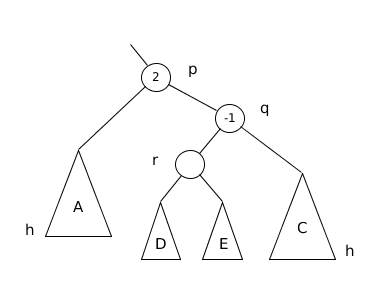
\includegraphics[scale=0.6]{imagenes/fig12.jpg}
	\end{center}
	\caption{$fb(p) = 2$ y $fb(q) = -1$}
	\label{fig12}
\end{figure}

Para distribuir el peso de $B$, necesitamos trasladar una parte de 'el hacia el sub'arbol derecho de $q$. Como podemos intuir a esta altura, es posible conseguir esto v'ia una \textsc{Right-Rotate}($q$). Dejamos como tarea para el lector verificar que esta sola esta rotaci'on puede no ser suficiente en ciertos casos, dependiendo del valor de $fb(r)$. Si ejecutamos la \textsc{Left-Rotate}($p$) pendiente, ahora s'i habremos restaurado el balanceo. El proceso se muestra en la figura \ref{fig13}.

\begin{figure}[H]
	\begin{center}
		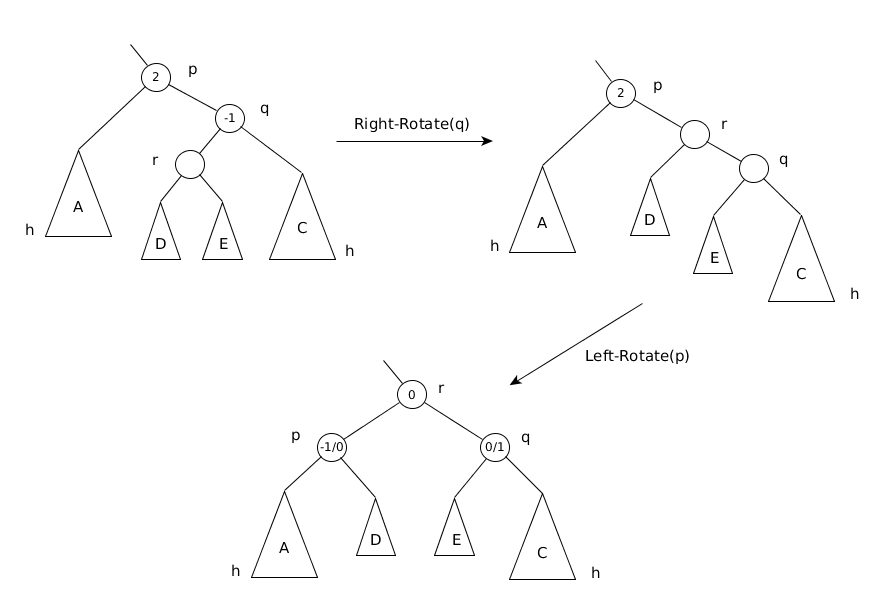
\includegraphics[scale=0.55]{imagenes/fig13.jpg}
	\end{center}
	\caption{$fb(p) = 2$ y $fb(q) = -1$ \textbf{(caso C)}}
	\label{fig13}
\end{figure}

Notemos que los factores de balanceo de $p$ y $q$ depender'an de las alturas de los sub'arboles $D$ y $E$. Si miramos el 'arbol original, el sub'arbol con ra'iz en $r$ ten'ia altura $h + 1$, con lo cual las alturas de $D$ y $E$ son algunas de $h - 1$ 'o $h$.

Hasta ahora estuvimos analizando el caso $fb(p) = 2$. El caso $fb(p) = -2$ es completamente sim'etrico, y no repetiremos el mismo an'alisis detallado. Las figuras \ref{fig14}, \ref{fig15} y \ref{fig16} muestran las rotaciones necesarias para cada uno de los casos, que son, siguiendo el mismo orden que antes, an'alogos.

\begin{figure}[H]
	\begin{center}
		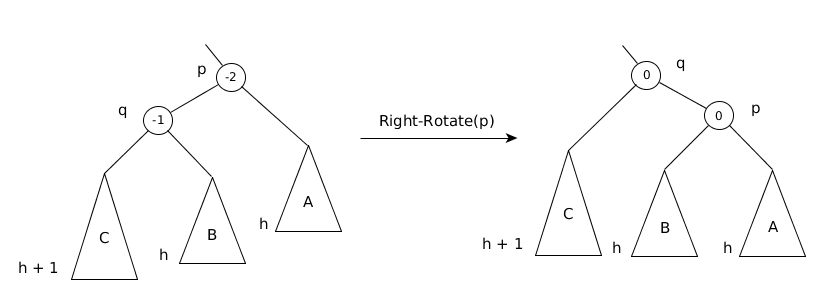
\includegraphics[scale=0.55]{imagenes/fig14.jpg}
	\end{center}
	\caption{$fb(p) = -2$ y $fb(q) = -1$ \textbf{(caso D)}}
	\label{fig14}
\end{figure}

\begin{figure}[H]
	\begin{center}
		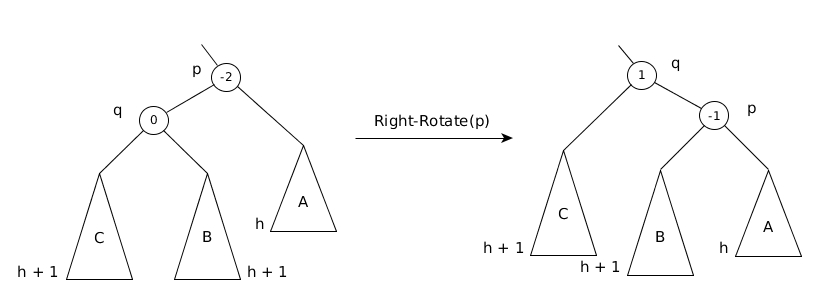
\includegraphics[scale=0.55]{imagenes/fig15.jpg}
	\end{center}
	\caption{$fb(p) = -2$ y $fb(q) = 0$ \textbf{(caso E)}}
	\label{fig15}
\end{figure}

\begin{figure}[H]
	\begin{center}
		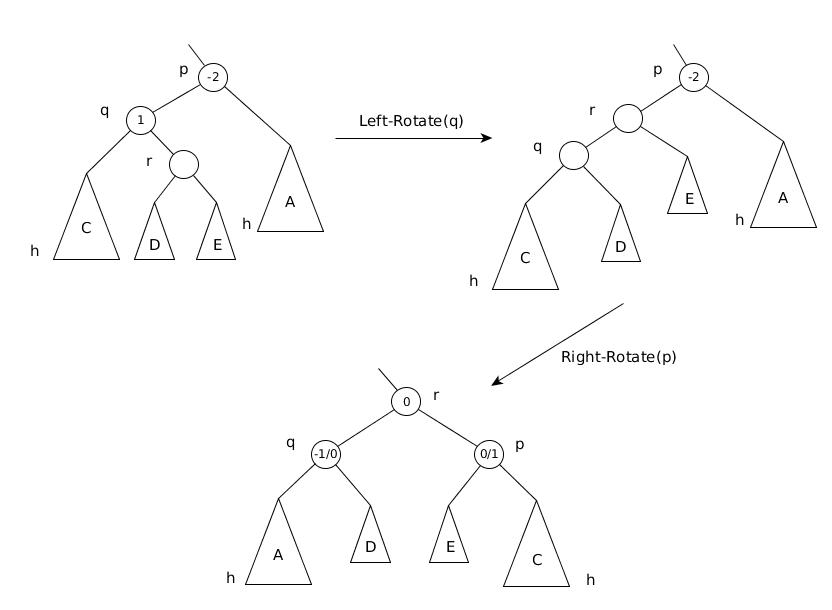
\includegraphics[scale=0.55]{imagenes/fig16.jpg}
	\end{center}
	\caption{$fb(p) = -2$ y $fb(q) = 1$ \textbf{(caso F)}}
	\label{fig16}
\end{figure}

\subsection{Inserci'on en un AVL}

Recordemos que la inserci'on en un AVL agrega un nuevo nodo como una hoja del 'arbol. Esto implica que s'olo pueden cambiar los factores de balanceo de nodos que se encuentren en el camino que entre la ra'iz y el nodo agregado. Si logramos rebalancear cada factor desbalanceado a lo largo de este camino, habremos reestablecido el balance en todo el 'arbol. Esta idea motiva el algoritmo de inserci'on sobre AVLs.

\SetKwFunction{inser}{AVL-Insert}

\begin{algorithm}
  	\DontPrintSemicolon
  	\inser{$T$, $k$}{\;

	\Begin{
		Insertar $k$ en $T$ como en un ABB\;
		Sea $x$ el nodo agregado\;
		\textsc{AVL-Rebalance}($T$, $x$)
 	}
 	}
\end{algorithm}

\SetKwFunction{reba}{AVL-Rebalance}

\begin{algorithm}
  	\DontPrintSemicolon
  	\reba{$T$, $x$}{\;

	\Begin{
		\ForEach {$p$ nodo en el camino entre $x$ y la ra'iz de $T$} {
			\If {$|fb(p)| > 1$} { 
				Rebalancear el sub'arbol con ra'iz en $p$ como en alguno de los casos A, ..., F 
			}
		}
 	}
 	}
\end{algorithm}

La complejidad del algoritmo es claramente proporcional a la altura del 'arbol, es decir, $O(\lg n)$.

La correctitud de este algoritmo se basa fuertemente en que cualquier desbalanceo que nos encontremos tendr'a la forma de alguno de los clasificados anteriormente. Es evidente que el primero de todos que nos encontremos, recorriendo el camino desde abajo, ser'a alguno de los vistos, puesto que el factor de balanceo no puede tener m'odulo mayor que 2, que a su vez se debe a que como s'olo insertamos un nodo, entonces a lo sumo aumentamos la altura de una rama en uno. Pero luego de hacer el primer rebalanceo, ¿por qu'e los factores de nodos superiores no empeoran a'un m'as? ¿No podr'ia pasar que alg'un factor de balanceo pase a tener m'odulo mayor que 2?

Para responder negativamente a esto, debemos analizar c'omo se propagan los cambios en la altura luego de efectuar el primer rebalanceo. Para esto, debemos tener en cuenta c'omo era la altura del sub'arbol a rebalancear, en el instante previo a la inserci'on, y cu'al es su altura luego del rebalanceo.

Hacemos el an'alisis para el rebalanceo del caso A, y dejamos el resto como ejercicio para el lector. 

\begin{teo}
Durante una inserci'on, si el primer rebalanceo es de tipo A, entonces, luego del mismo, ning'un nodo en el camino entre la ra'iz del sub'arbol rebalanceado y la ra'iz de todo el 'arbol tendr'a un factor de balanceo de m'odulo mayor que dos.

\begin{proof}
Utilizamos la notaci'on de la figura \ref{fig9}. Sea $P$ el sub'arbol con ra'iz en $p$, previo a la inserci'on. Sea $Q$ el resultado de insertar y efectuar el primer rebalanceo (de tipo A) en ese sub'arbol. En este caso, la inserci'on se debe haber producido necesariamente en el sub'arbol $C$ (¿por qu'e?), y la altura de $P$ es $h + 2$. Como la altura de $Q$ tambi'en es $h + 2$, entonces ning'un factor de balanceo de un nodo en el camino entre la ra'iz de $Q$ y la ra'iz del 'arbol pudo haber cambiado respecto de su valor previo a la inserci'on.
\end{proof}
\end{teo}

Observar que este resultado muestra algo m'as fuerte que lo que quer'iamos. Hemos probado que, en una inserci'on, si el primer rebalanceo es de tipo A, luego del mismo todo el 'arbol queda balanceado. Se puede demostrar que, luego de una inserci'on, los 'unicos casos de rebalanceo que se pueden dar son A, C, D y F, y que luego de realizar alguno de ellos, todos los factores de balanceo quedan reestablecidos.

\subsection{Borrado en un AVL}

Recordemos que los casos de borrado en un ABB son tres, que dependen de la cantidad de hijos del nodo a borrar. Llamemos $z$ al nodo a borrar.

Si $z$ no tiene hijos, entonces es borrado y el resto del 'arbol no cambia. Esto s'olo puede generar variaciones de a lo sumo una unidad en los factores de balanceo de los nodos del camino entre el padre de $z$ y la ra'iz.

Si $z$ tiene un 'unico hijo, entonces ese hijo es conectado con el padre de $z$. Al igual que antes, s'olo pueden cambiar en uno, los factores de nodos entre el padre de $z$ y la ra'iz.

Por 'ultimo, si $z$ tiene dos hijos, $z$ es reemplazado por el nodo antecesor (o el sucesor) en el sub'arbol del cual es ra'iz. En otras palabras, se reemplaza $z$ por el nodo de clave m'axima en su sub'arbol izquierdo, al que llamamos $x$, y al 'unico hijo de $x$ se lo conecta con el padre de $x$, salvo cuando $x$ es el hijo izquierdo de $z$, en cuyo caso el hijo de $x$ conservar'a su relaci'on con $x$. Por ende, s'olo cambiar'an los factores de balanceo de los nodos entre el antiguo padre de $x$ (si $x$ no es hijo de $z$) o bien $x$ mismo (en caso contrario), y la ra'iz del 'arbol.

Este argumento muestra que, al igual que en la inserci'on, el borrado de nodos s'olo modifica, a lo sumo en una unidad, los factores de balanceo de nodos entre cierto nodo particular (que depende del caso de borrado) y la ra'iz.

%\newpage

\SetKwFunction{dele}{AVL-Delete}

\begin{algorithm}
  	\DontPrintSemicolon
  	\dele{$T$, $k$}{\;

	\Begin{
		Borrar $k$ de $T$ como en un ABB\;
		Sea $x$ primer nodo posiblemente desbalanceado\;
		\textsc{AVL-Rebalance}($T$, $x$)
 	}
 	}
\end{algorithm}

El costo de este algoritmo tambi'en es proporcional a la altura del 'arbol, o sea, $O(\lg n)$.

Al igual que en la inserci'on, el algoritmo se basa en que nunca aparecer'a un nodo desbalanceado con un factor de balanceo de m'odulo mayor que 2, pero no daremos una prueba formal de que esto efectivamente ocurre.

En el caso del borrado, cualquiera de los seis casos de rebalanceo puede darse, y el desbalance puede propagarse hacia nodos superiores, a'un luego de haber efectuado una operaci'on de rebalanceo. Por este motivo, no es posible cortar anticipadamente el recorrido hacia la ra'iz, luego del primer rebalanceo, como s'i era posible en la inserci'on.


\section{Conclusi'on}

Organizar la informaci'on utilizando ABBs balanceados permite acceder a ella eficientemente. Este r'apido acceso se torna imprescindible cuando el vol'umen de informaci'on que debemos manejar es enorme. Sin embargo, lograr el balanceo no es una tarea sencilla, y para conseguirlo necesitamos imponer ciertas restricciones que sean sostenibles a lo largo de las modificaciones que se efect'uen sobre el 'arbol.

Hemos explorado distintos criterios para forzar el balanceo de un 'arbol, observando que algunos de ellos son demasiado r'igidos como para poder ser mantenidos. El balanceo en altura prob'o ser efectivo en ese sentido. Queda claro que podr'ia haber otras alternativas para llegar al preciado balanceo, y de hecho las hay, como por ejemplo aquellas utilizadas por los 'arboles red-black, 'arboles B o 'arboles 2-3-4. Si bien todas estas estructuras cumplen con el objetivo de almacenar en orden y en forma balanceada toda la informaci'on, no todos son igualmente complejos: la distinta rigidez entre los criterios de balanceo que utilizan hace que la dificultad de los algoritmos de cada estructura y, a nivel de eficiencia, la cantidad de rebalanceos que necesitan, var'ie entre ellas. El balanceo de 'arboles, por lo tanto, no es s'olo un concepto utilizado por los 'arboles AVL, sino que tiene la jerarqu'ia de un campo de estudio en computaci'on.

\nocite{*}

\bibliographystyle{plain}
\bibliography{main}

\end{document}
